\section{Network Architecture}

The model consists of

\begin{itemize}
    \item Batch size 
    \item skdfj
    \item sdfk
\end{itemize}

\begin{table}[h]
    \centering
    \begin{tabular}{ l c r }
      \hline
      Layer (type) & Output shape & Param \# \\ \hline
      lstm\_1 (LSTM) & (None, 10, 256) & 1234678 \\ \hline
      lstm\_1 (LSTM) & (None, 10, 256) & 1234678 \\ \hline
      lstm\_1 (LSTM) & (None, 10, 256) & 1234678 \\ \hline
      lstm\_1 (LSTM) & (None, 10, 256) & 1234678 \\ \hline
      lstm\_1 (LSTM) & (None, 10, 256) & 1234678 \\ \hline
      Total params: & & \\
      Trainable params: & & \\ 
      Non-Trainable params: 0 & & \\ \hline
      
    \end{tabular}
    \caption{Parameters for our architecture}
    \label{tab:archparams}
\end{table}


\begin{figure}[h]
    \centering
    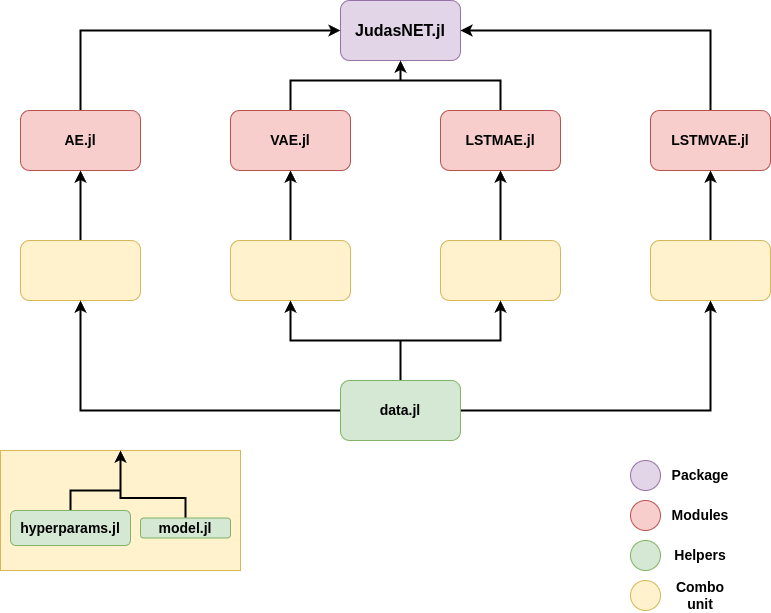
\includegraphics{figures/judasnet.png}
    \caption{JudasNET network architecture}
    \label{fig:judasnet}
\end{figure}


\subsection{Hyperparameters}

See \cite{app:hyperparams} for a detailed view on all the different hyperparameters used for this particular model

